\documentclass[varwidth=40cm]{standalone}
\usepackage{tikz}
\usetikzlibrary{patterns,decorations.pathreplacing}
\usepackage{style}

\begin{document}
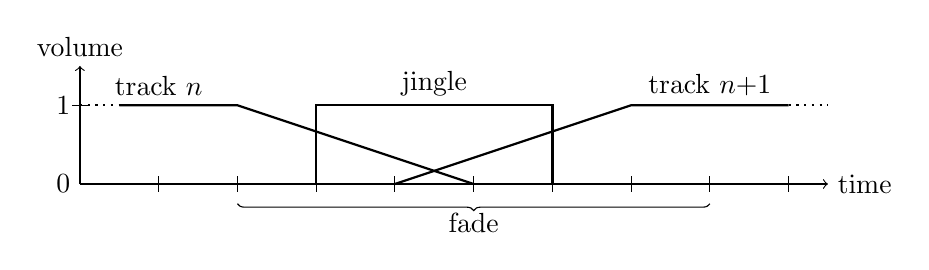
\begin{tikzpicture}
  \draw[->] (0,0) -- (0,1.5) node[above]{volume};
  \draw (-0.1,1) -- (0.1,1);
  \draw (0,1) node[left]{1};
  \draw (0,0) node[left]{0};
  \draw[->] (0,0) -- (9.5,0) node[right]{time};
  \foreach \x in {1,2,3,4,5,6,7,8,9} \draw (\x,-0.1) -- (\x,0.1);
  \draw[thick,dotted] (0,1) -- (.5,1);
  \draw[thick] (.5,1) -- (2,1) -- (5,0);
  \draw[thick] (3,0) -- (3,1) -- (6,1) -- (6,0);
  \draw[thick] (4,0) -- (7,1) -- (9,1);
  \draw[thick,dotted] (9,1) -- (9.5,1);
  \draw (4.5,1) node[above] {jingle};
  \draw (1,1) node[above]{track $n$};
  \draw (8,1) node[above]{track $n{+}1$};
  \draw [decoration={brace,mirror}, decorate] (2,-.25) -- (8,-.25) node [pos=0.5,below] {fade};
\end{tikzpicture}
\end{document}
